\documentclass[letterpaper, 11pt]{article}
%\usepackage[hmargin = 1in, vmargin = 1in]{geometry}
\usepackage{amsmath}
\usepackage{amssymb}
\usepackage{enumitem}
\usepackage{mathrsfs}
\usepackage{tikz}
\usepackage{graphicx}
\usepackage{algorithmicx}
\usepackage{algpseudocode}
\usepackage{microtype}
% \doublespacing
\setlength{\headheight}{14pt}
\usepackage{fancyhdr}
\pagestyle{fancy}
\rhead{Gabriel Wallace}
\lhead{Comp Sci 3130}

\newcommand{\card}{\text{Card}}
\newcommand{\N}{\mathbb{N}}
\newcommand{\R}{\mathbb{R}}
\newcommand{\Z}{\mathbb{Z}}
\newcommand{\Q}{\mathbb{Q}}

\newcommand{\inv}{^{-1}}
\newcommand{\abs}[1]{\lvert #1 \rvert}
\newcommand{\hwnumber}[3]{\medskip \noindent\textbf{#1.} Section #2 \##3 \smallskip}
\newcommand{\Mod}[1]{\ \mathrm{mod}\ #1}

\begin{document}
\begin{center}
	{\LARGE Project 1}\\
\end{center}

\section*{Theoretical Analysis}
We have two algorithms to find the \(n\)th Fibonacci number, \(F_n\), one recursive and
one iterative. We proceed with the theoretical analysis of these two
algorithms, and find the order of growth of each.

\subsection*{Recursive algorithm}
We have the following recursive definition for \(F_n\): 
\[F(n) = F(n - 1) + F(n - 2) \]
To find the general form for \(F(n)\), we solve a linear homogenous recurrence
relation, and have
\[F(n) = \frac{1}{\sqrt{5}}(\varphi) ^ n - 
\frac{1}{\sqrt{5}} (\hat{\varphi}) ^ n\]
with
\[\varphi = \left(\frac{1 + \sqrt{5}}{2} \right) \text{ and } 
\hat{\varphi} = \left(\frac{1 - \sqrt{5}}{2} \right)\]

To find the order of growth of \(F(n)\), we need to calculate the limit as
\(n\) approaches infinity. Since \(\abs{\hat{\varphi}} \approx 0.62 < 1\), then
\[\lim_{n \to \infty} \frac{1}{\sqrt{5}} (\hat{\varphi})^n = 0.\]
And since, \(\abs{\varphi} \approx 1.62 > 1\), then 
\[\lim_{n \to \infty} \frac{1}{\sqrt{5}} (\varphi)^n = \infty.\]
So,
\[\lim_{n \to \infty} F(n) = \frac{1}{\sqrt{5}}\lim_{n \to \infty}(\varphi)^n +
(\hat{\varphi})^n = \frac{1}{\sqrt{5}}\lim_{n \to \infty}(\varphi)^n = \infty.\]

\medskip

Thus, \(F(n) \in \Theta(\varphi^n)\) or \(F(n) \in \mathcal{O}(2^n)\)

\subsection*{Iterative algorithm}
We have the following pseudocode of the iterative algorithm from the book on
page 82:

\medskip
\noindent\textbf{ALGORITHM} \(Fib(n)\)
\begin{algorithmic}
    \State //Computes the nth Fibonacci number iteratively by using its definition
    \State //Input: A nonnegative integer \(n\)
    \State //Output: The \(n\)th Fibonacci number
    \State \(F[0] \gets 0, F[1] \gets 1\)
    \For {\(i \gets 2 \textbf{ to } n\)}
    \State \(F[i] \gets F[i - 1] + F[i - 2]\)
    \EndFor
    \State\Return \(F[n]\)
\end{algorithmic}
\medskip

The first two assignments to \(F[0]\) and \(F[1]\) are of constant time, so the
efficiency of the algorithm is dependent on the \textbf{for} loop. Since the 
operation that occurs on every iteration of the loop is addition, which can be
completed in constant time, we have
\[C(n) = \sum_{i = 2}^{n} 1 = (n - 2 + 1) = n - 1\]

So \(C(n) \in \Theta(n)\)

\newpage

\section*{Empirical Analysis}
Running the code from part (C), we have created two csv files
\texttt{iterative.csv} and \texttt{recursive.csv} for the respective
algorithms. We use the R programming language to create two plots of results
from part (C). We have the raw data in the black dots, and then a calculated
trendline in blue.  

\begin{figure}[h]
    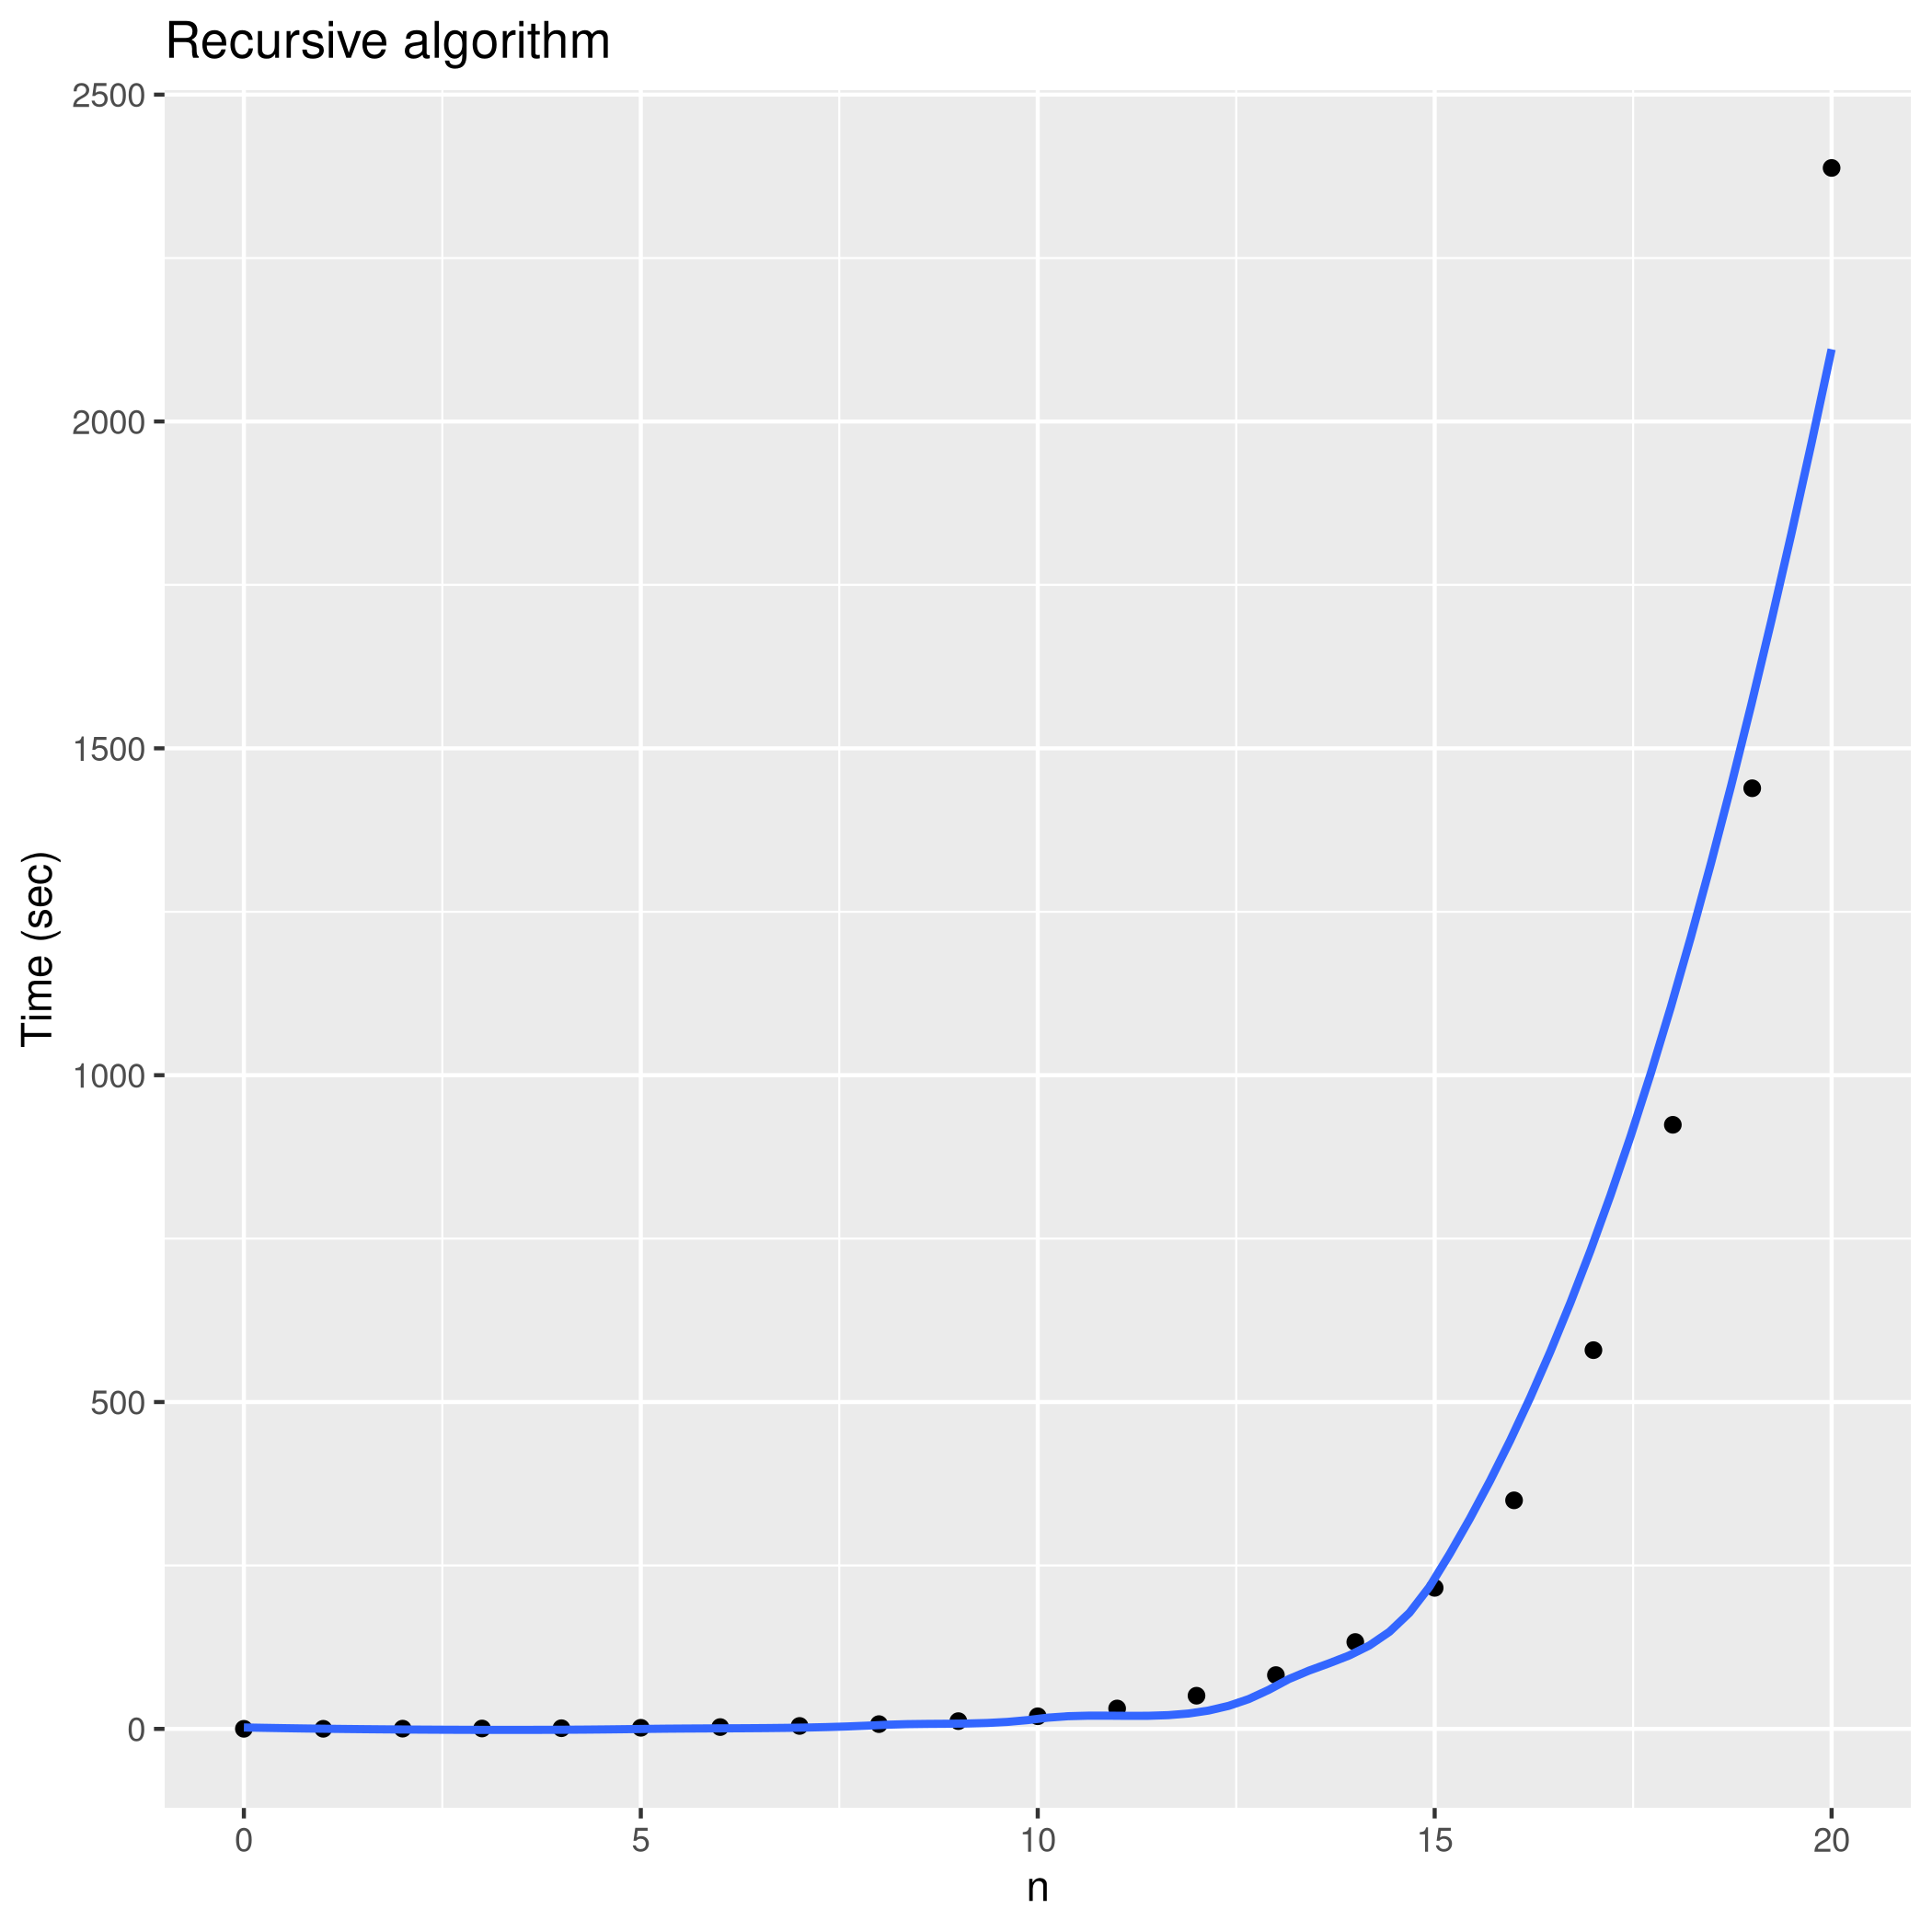
\includegraphics[width=\linewidth]{iterative_plot.png}
\end{figure}

\begin{figure}[h]
    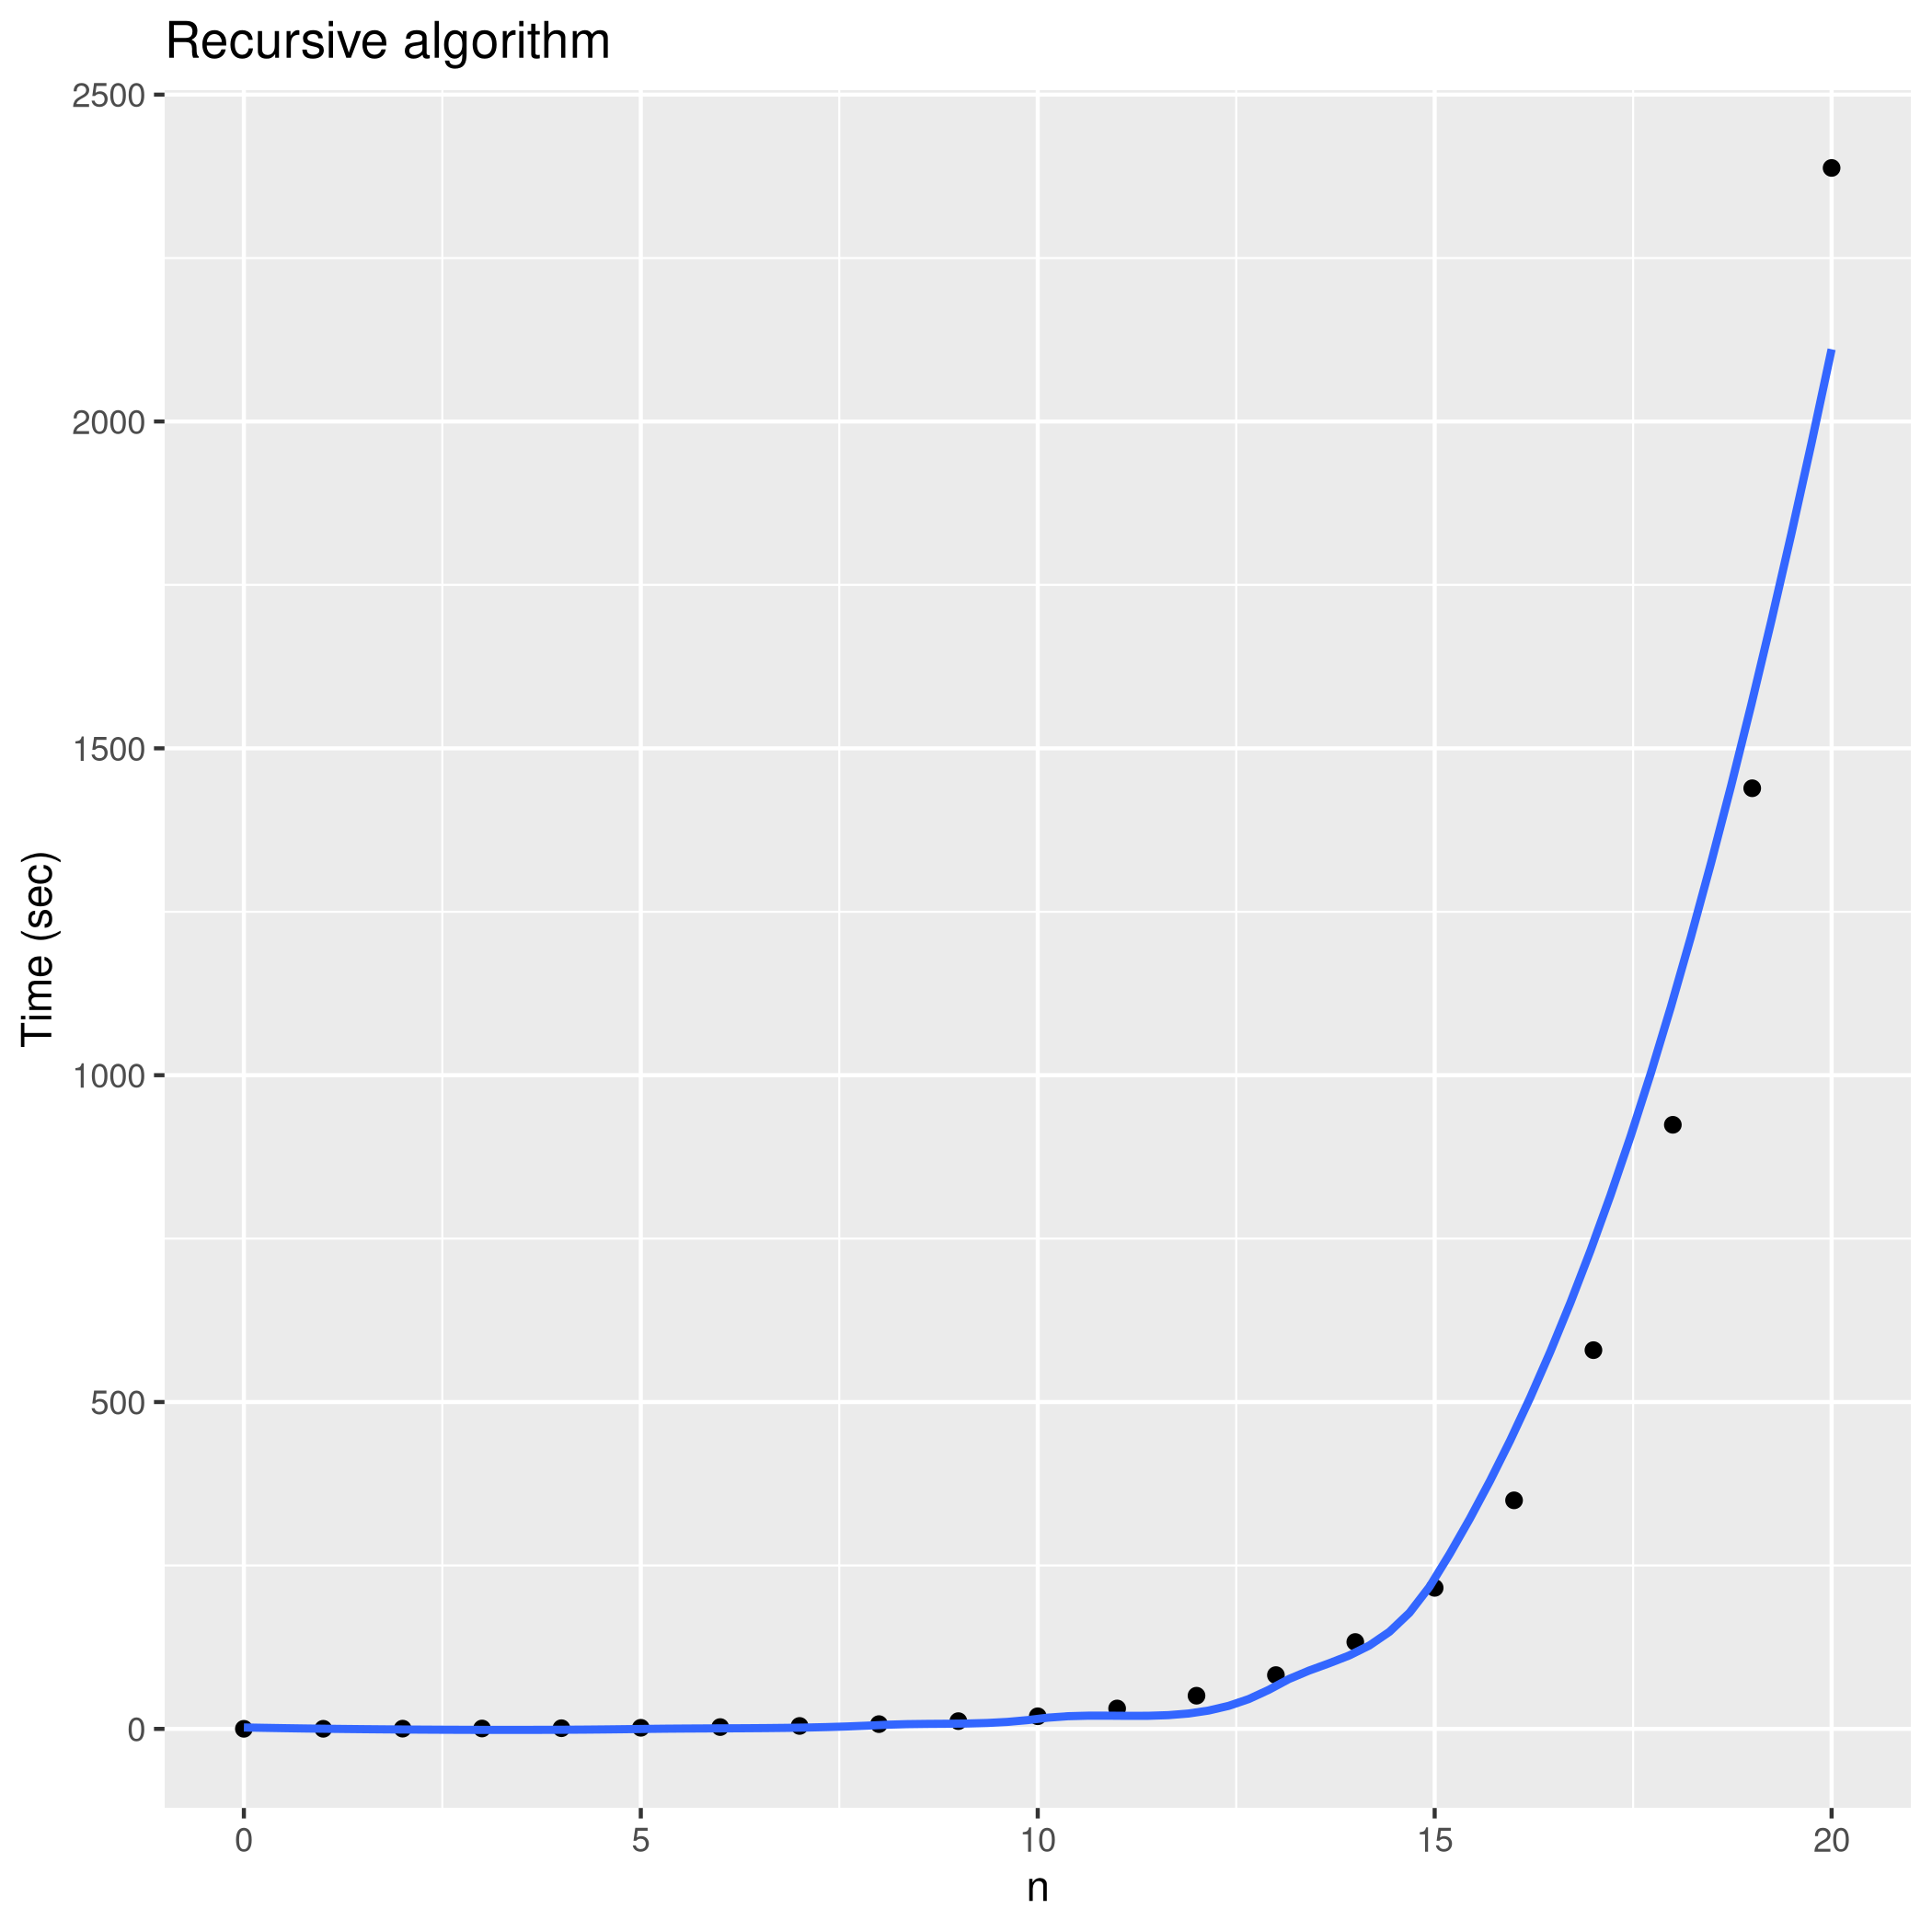
\includegraphics[width=\linewidth]{recursive_plot.png}
\end{figure}

From these plots, we can see that our theoretical analysis is correct. The
iterative and recursive algorithms have orders of growth of linear and
exponential time respectively. 

\end{document}
